\subsection{Halved Model}


\begin{figure}
    \centering
    \subfloat[The full model]{
        \includegraphics[width=.4 \textwidth]{62_MinimalRepr_Adding/2D_Period_1_Zoomed/result.png}
    }
    \subfloat[The halved model]{
        \includegraphics[width=.4 \textwidth]{63_MinimalRepr_Adding_Halved/2D_Period_1_Zoomed/result.png}
    }
    \caption{2D period scans of the same model in two versions}
    \label{fig:minrep.adding1.corner.period}
\end{figure}

\begin{figure}
    \centering
    \subfloat[The full model]{
        \includegraphics[width=.4 \textwidth]{62_MinimalRepr_Adding/1D_Period_1_add_hor_D1/result.png}
    }
    \subfloat[The halved model]{
        \includegraphics[width=.4 \textwidth]{63_MinimalRepr_Adding_Halved/1D_Period_1_add_hor_D1/result.png}
    }
    \caption{1D period scans of the same model in two different versions. The parameter range is marked red in \Cref{fig:minrep.adding1.corner.period}}
\end{figure}